% (The MIT License)
%
% Copyright (c) 2023-2024 Yegor Bugayenko
%
% Permission is hereby granted, free of charge, to any person obtaining a copy
% of this software and associated documentation files (the 'Software'), to deal
% in the Software without restriction, including without limitation the rights
% to use, copy, modify, merge, publish, distribute, sublicense, and/or sell
% copies of the Software, and to permit persons to whom the Software is
% furnished to do so, subject to the following conditions:
%
% The above copyright notice and this permission notice shall be included in all
% copies or substantial portions of the Software.
%
% THE SOFTWARE IS PROVIDED 'AS IS', WITHOUT WARRANTY OF ANY KIND, EXPRESS OR
% IMPLIED, INCLUDING BUT NOT LIMITED TO THE WARRANTIES OF MERCHANTABILITY,
% FITNESS FOR A PARTICULAR PURPOSE AND NONINFRINGEMENT. IN NO EVENT SHALL THE
% AUTHORS OR COPYRIGHT HOLDERS BE LIABLE FOR ANY CLAIM, DAMAGES OR OTHER
% LIABILITY, WHETHER IN AN ACTION OF CONTRACT, TORT OR OTHERWISE, ARISING FROM,
% OUT OF OR IN CONNECTION WITH THE SOFTWARE OR THE USE OR OTHER DEALINGS IN THE
% SOFTWARE.

\documentclass{article}
\usepackage{../osbp}
\newcommand*\thetitle{Releasing}
\begin{document}

\plush{\osbpTitlePage{7}{}}

\qte
  [\nospell{Andre Van Der Hoek}]
  {andre-van-der-hoek}
  {Simply \ul{making available} and retrieving interdependent components individually \ul{neither} facilitates independent software development \ul{nor} encourages widespread use of large systems of systems.}
  {van1997software}

\qte
  [\nospell{G{\"u}nther Ruhe}]
  {gunther-ruhe}
  {Release planning is typically done \textit{ad hoc} and \ul{not} based on sound \ul{models and methodologies}. This is even the case when planning involves several hundred features.}
  {ruhe2005art}

\thought{Release when it's different, not when it's good.}

\qte
  [\nospell{Kazu Okumoto}]
  {kazu-okumoto}
  {\textbf{\nospell{Goel-Okumoto} model}: An important problem of practical concern is the determination of the point when testing should \ul{stop} and the system can be considered ready for release, that is, the determination of the \ul{software release time}. Two criteria are investigated: software reliability and total expected cost.}
  {okumoto1979optimum}

\qte
  [\nospell{Shigeru Yamada}]
  {shigeru-yamada}
  {This paper extends the problem of \citet{okumoto1979optimum} by evaluating \ul{both criteria} simultaneously. We discuss optimal software release policies which minimize a total average software cost under the constraint of satisfying a software reliability requirement.}
  {yamada1985cost}
\pitch{
  \begin{multicols}{2}
  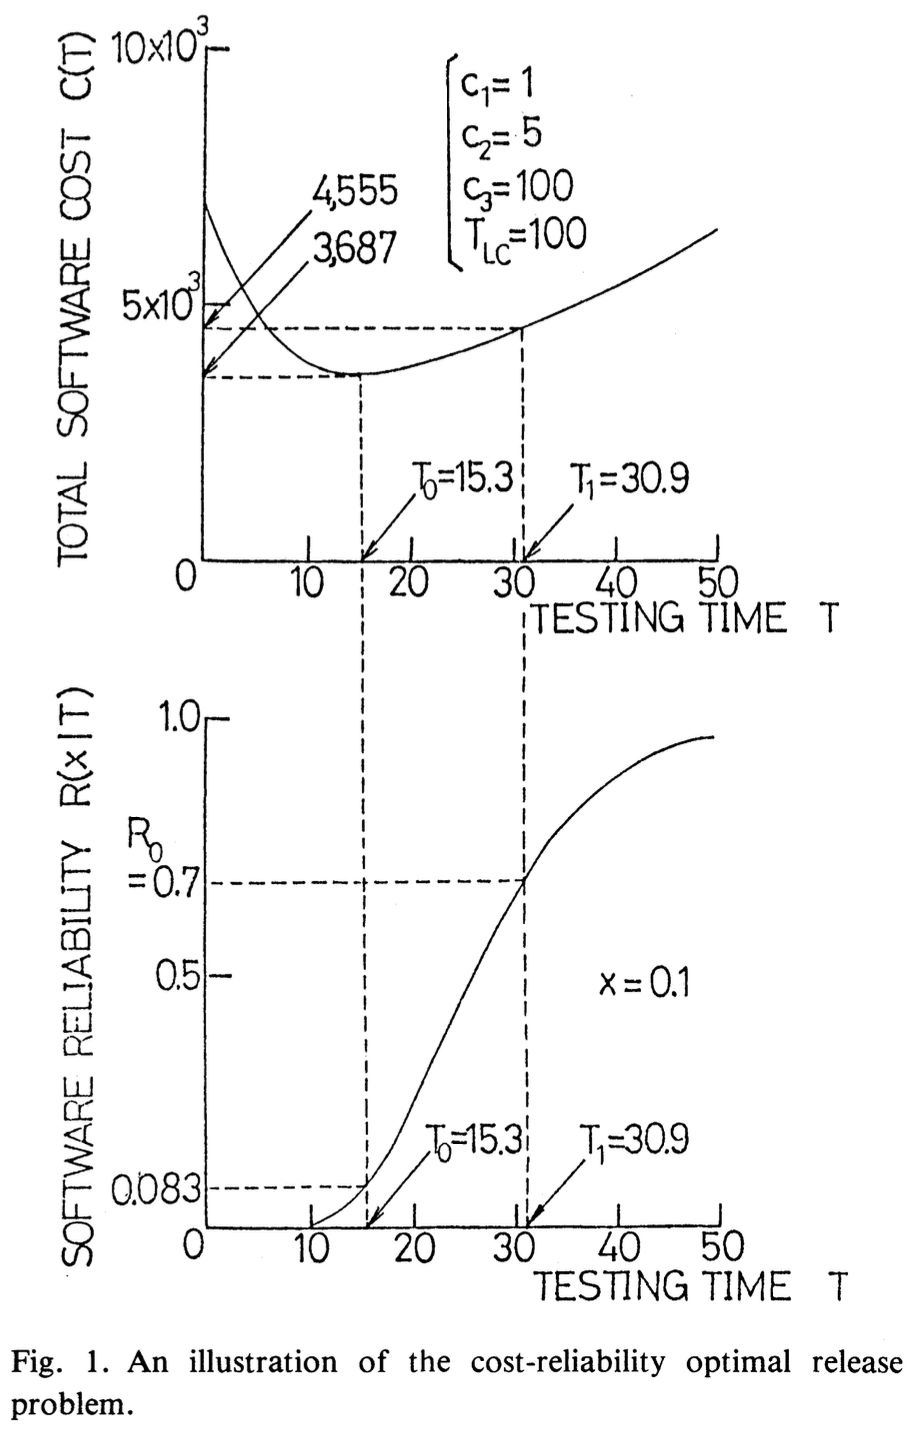
\includegraphics[width=.65\linewidth]{time-vs-cost.png}
  \par\columnbreak\par
  ``The optimum software release time is the testing time which comes closest to satisfying some pre-specified software reliability.''
  \source{yamada1985cost}
  \end{multicols}}

\qte
  [\nospell{Nasif Imtiaz}]
  {nasif-imtiaz}
  {We find that the open source packages are typically fast in releasing security fixes, as the median release comes within \ul{4 days} of the corresponding security fix. However, 25\% of the releases still have a delay of at least \ul{20 days}.}
  {imtiaz2022open}

\thought{Fully automate the release process, avoiding any manual intervention.}

\qte
  [\nospell{Jez Humble}]
  {jez-humble}
  {Over time, deployments should tend towards being fully automated. There should be \ul{two tasks} for a human being to perform to deploy software into a development, test, or production environment: to pick the version and environment and to press the `deploy' button.}
  {humble2010continuous}

\thought{Release frequently.}

\qte
  [\nospell{Victor Basili}]
  {victor-basili}
  {If improving productivity is the main concern, then it may be wise to try to \ul{avoid} scheduling \ul{small} error correction releases. Instead the manager should try, when possible, to \ul{package} small error corrections in a release with larger enhancements.
  \pptPin{\raggedleft\colorbox{red}{\color{white}Respectfully} \\ \colorbox{red}{\color{white}disagree!}\par}}
  {basili1996understanding}

\qte
  [\nospell{Foutse Khomh}]
  {foutse-khomh}
  {We found that (1)~with shorter release cycles, users do not experience significantly more post-release bugs and (2)~bugs are fixed faster, yet (3)~users experience these bugs earlier during software execution (the program crashes earlier).}
  {khomh2012faster}

\thought{Use SemVer.}

\pitch{
  \begin{multicols}{2}
  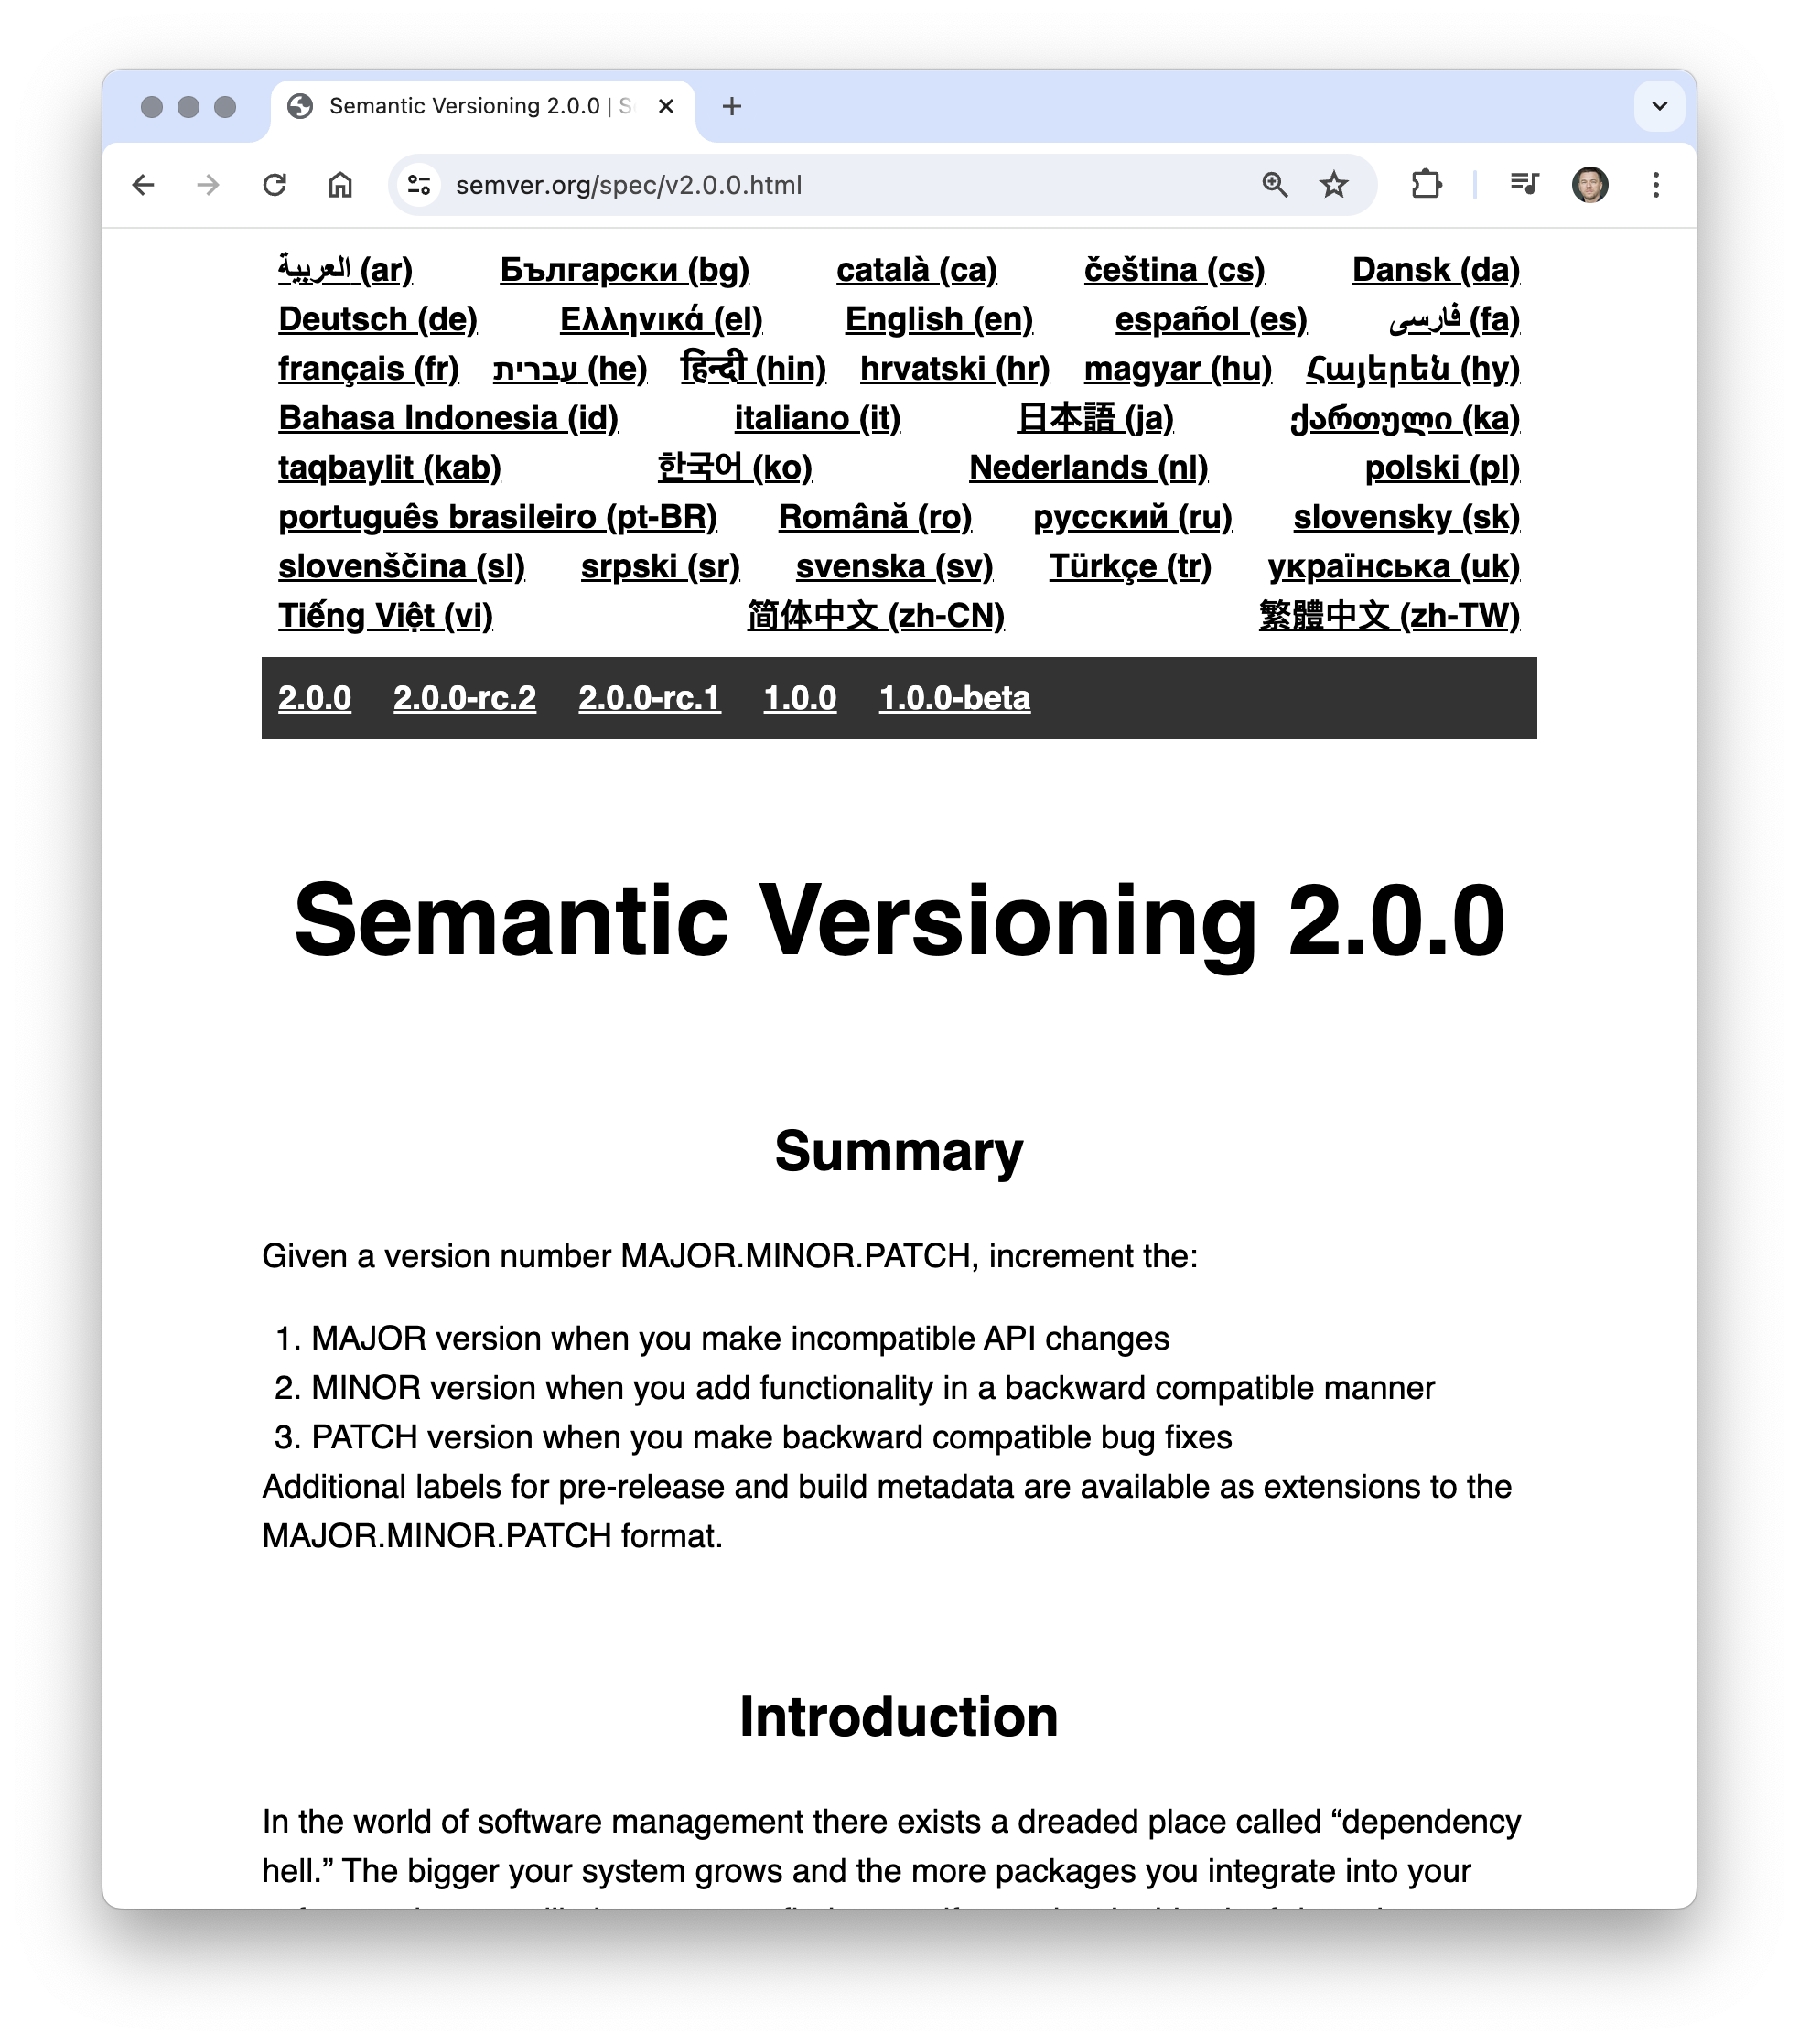
\includegraphics[width=.9\linewidth]{semver.png}
  \par\columnbreak\par
  ``The implication of semantic versioning is that clients may rely on dependencies subject to flexible version constraints, like \texttt{1.2.*}. Such a client may safely upgrade to new micro versions (e.g., from \texttt{1.2.3} to \texttt{1.2.4}), fully automated.''
  \source{lam2020putting}
  \end{multicols}}

\thought{Generate release notes automatically.}

\pitch{
  \begin{multicols}{2}
  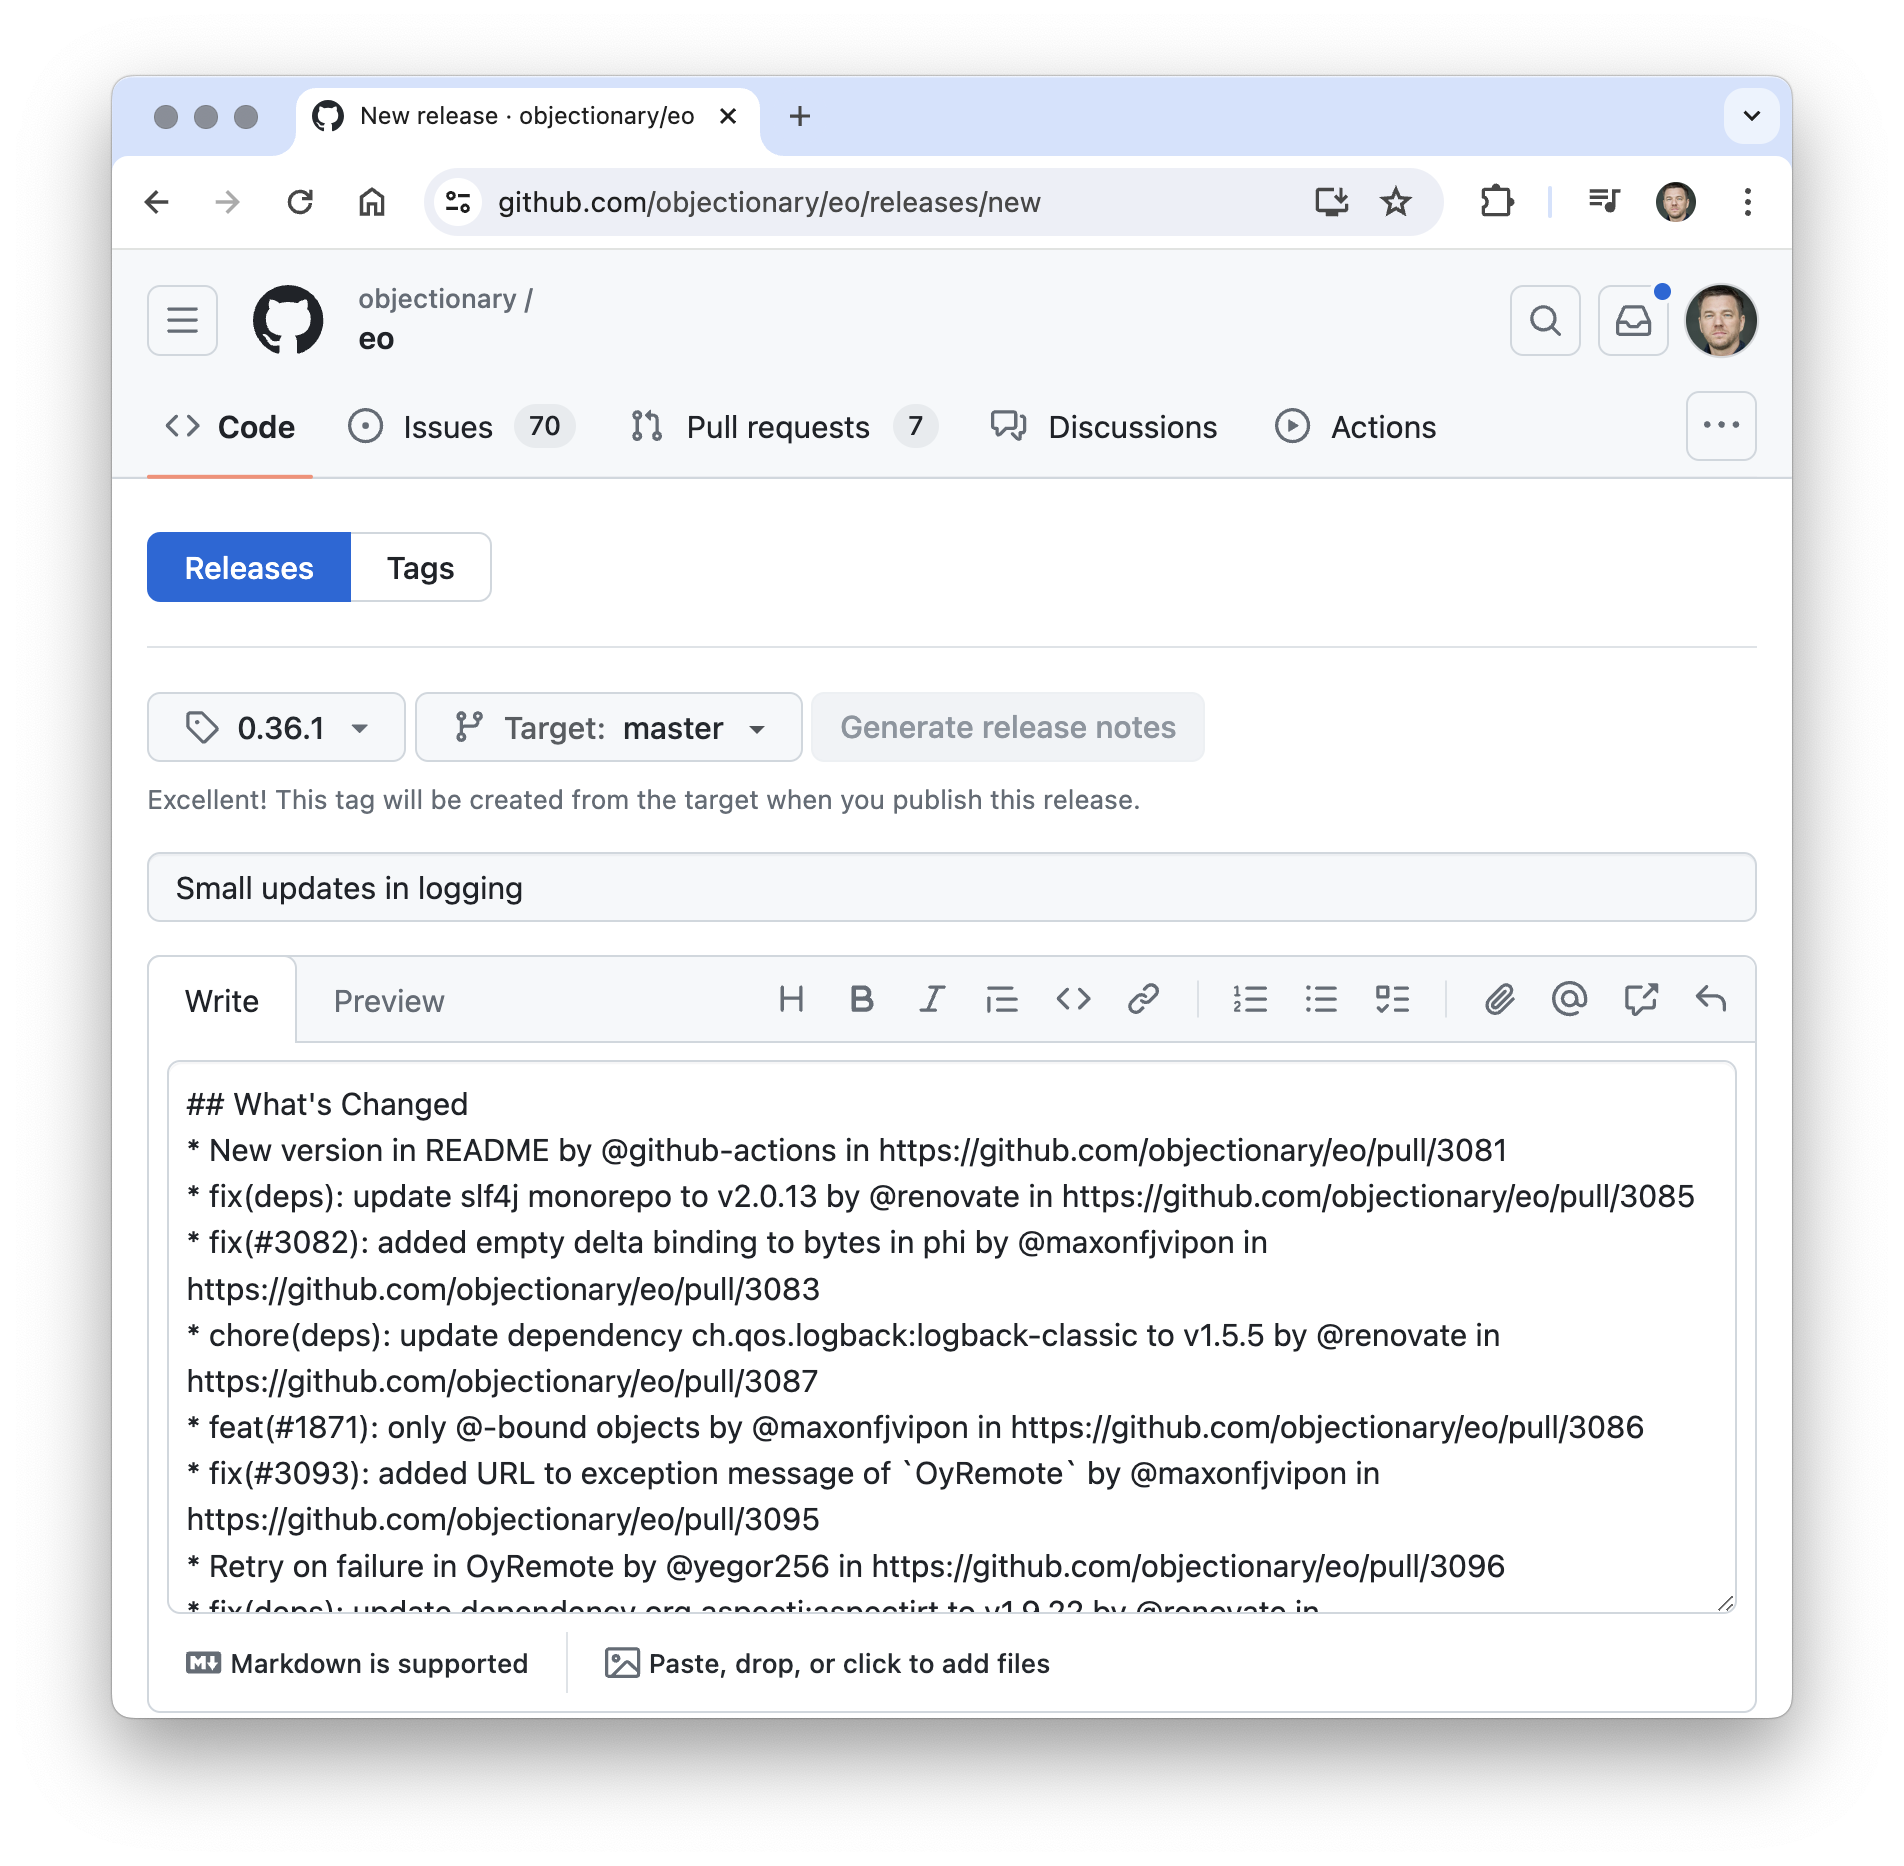
\includegraphics[width=.9\linewidth]{notes.png}
  \par\columnbreak\par
  ``Automatically generated release notes provide an automated alternative to manually writing release notes for your GitHub releases. With automatically generated release notes, you can quickly generate an overview of the contents of a release.''
  {\par\scriptsize\url{https://docs.github.com/en/repositories/releasing-projects-on-github/automatically-generated-release-notes}\par}
  \end{multicols}}

\pitch{
  \pptBanner{Some Release Notes Generators:}
  \begin{itemize}\setlength\itemsep{0em}
    \item \href{https://clickup.com/features/ai/release-notes-generator}{ClickUp}
    \item \href{https://www.taskade.com/generate/programming/release-notes}{Taskade}
    \item \href{https://zeda.io/feature/release-note-ai}{Zeda}
    \item \href{https://www.aha.io/blog/introducing-ai-powered-release-notes}{Aha}
    \item \href{https://www.releasesnotes.dev/}{ReleasesNotes}
    \item \href{https://scribehow.com/tools/product-release-note-generator}{ScribeHow}
    \item \href{https://www.released.so/}{Released}
    \item \href{https://github.com/marketplace/ai-github-release-notes}{ai-github-release-notes}
  \end{itemize}
  {\scriptsize Try Google search with ``generate release notes with AI''\par}}

\qte
  [\nospell{Jianyu Wu}]
  {jianyu-wu}
  {We find that: 1) RN producers are more likely to miss information than to include incorrect information, especially for breaking changes; 2) improper layout may bury important information and confuse users; 3) many users find RNs inaccessible due to link deterioration, lack of notification, and obfuscate RN locations; 4) automating and regulating RN production remains challenging despite the great needs of RN producers.}
  {wu2022demystifying}

\thought{Publish binaries.}

\thought{Be aware of malware and protestware.}

\qte
  [\nospell{Marc Cheong}]
  {marc-cheong}
  {By providing guidance on ethical decision making and highlighting alternative methods for expressing concerns, ethics education can play a vital role in promoting a more balanced and responsible approach to protestware within the FOSS community.}
  {cheong2023ethical}

\thought{Announce them.}

\end{document}
